\documentclass{article}
\textwidth 6.5in \oddsidemargin .06in \evensidemargin .06in
\textheight 8.5in \topmargin -.6in
\usepackage{amsmath}
\usepackage{amsfonts}
\usepackage{amsthm}
\usepackage{cases}
\usepackage[breakable]{tcolorbox}
\usepackage{bm}
\usepackage[inkscapelatex=false]{svg}
\usepackage{ctex}
\usepackage{latexsym,wrapfig,picinpar}
\usepackage{amssymb}
\usepackage{soul}
\usepackage{graphicx}
\usepackage{amsmath,amsfonts}
\usepackage{mathrsfs}
\usepackage{epsfig,latexsym}
%\usepackage{alertmessage}
\usepackage{amsmath}
\usepackage{amssymb}
\usepackage{changes}
\usepackage{fancyref}
\usepackage{epsfig}
\usepackage{dcolumn}
\usepackage{CJK}
\usepackage{color}
%\usepackage{picins}
\usepackage{pstricks}
\usepackage{epstopdf}
\usepackage{array}

\newtheorem{remark}{Remark}[section]
\newtheorem{Lemma}{Lemma}[section]
\newtheorem{Corollary}{Corollary}[section]
\newtheorem{Theorem}{Theorem}[section]
\newtheorem{Proposition}{Proposition}[section]
\newtheorem{Definition}{Defintion}[section]
\renewcommand{\theequation}{\arabic{section}.\arabic{equation}}
\newcommand{\bb}[1]{{\mathbb #1}}
\newcommand{\E}{{\mathbb{E}}}
\newcommand{\N}{{\mathbb{N}}}
\newcommand{\R}{{\mathbb{R}}}
\newcommand{\Y}{{\mathbb{P}}}
\newcommand{\F}{{\mathcal{F}}}
\newcommand{\A}{{\mathcal{A}}}
\newcommand{\nn}{{\nonumber}}
\newcommand{\D}{{\mathrm{d}}}
\newcommand{\G}{{\mathcal{G}}}
\newcommand{\FF}{{\mathbb{F}}}
\newcommand{\GG}{{\mathbb{G}}}
\newcommand{\Q}{{\mathbb{Q}}}
\newcommand{\DD}{{\mathcal{O}}}
\newcommand{\x}{{\mathbf{x}}}
\newcommand{\y}{{\mathbf{y}}}
\newcommand{\h}{{\mathcal{H}}}
\newcommand{\K}{{\mathbf{k}}}
\newcommand{\s}{{\mathcal{S}}}
\newcommand{\DDD}{{\mathcal{D}}}
\newcommand{\w}{{\mathbf{w}}}
\newcommand{\YY}{{\mathcal{P}}}
\newcommand{\cad}{\textit{c\`{a}dl\`{a}g}}
\newcommand{\upcite}[1]{\textsuperscript{\cite{#1}}}
\newcommand{\expp}[1]{\mathop {\mathrm{e}^{ #1}}}












\allowdisplaybreaks
\linespread{1.5}






\begin{document}
\title{收入预测问题} 
%\author{ 张南怡\footnote{Corresponding author. Email: %nymath@163.com}}
\date{}
\maketitle
\begin{abstract}
	This paper proposes an intensity-based model to price spread options with default risk. Default risk is captured by a Cox process, whose intensity process is correlated with the volatility (two underlying assets). In addition, a general correlation between the intensity and  the volatility (two underlying assets) is allowed. We obtain an analytical expression of approximated prices of vulnerable spread options using the probability measure-change method. Finally, numerical examples are performed to demonstrate the accuracy of the approximation and illustrate the effect of  default risk.\\ \ \\
	{\bf Keywords}: Vulnerable Spread Options; Intensity-based Model; Default Risk; Cox Process.\\ \\
	{\bf JEL classification}: G13
	
	
\end{abstract}

\newpage
\section{Introduction}
回归,或者预测问题,本质在于求解条件期望。以单变量情形为例,
$$
Y(\omega) = E(Y|X)(\omega) + u(\omega).
$$
其中$E(Y|X=x)$可以记作$h(x)$,由于$h(x)$的形式未知,所以我们无法给出具体的形式。通常我们假定$h(x)$具有仿射结构,此时模型也称作一元线性回归。更一般的,我们可以利用多项式去估计$h(x)$,这样做的理由是Laurent展开定理。

\begin{Theorem}[Laurent Series]{\label{LS}} 
Suppose $f$ is analytic at an annulus of $z_0$, then f can be expressed as follows
$$
f(z) = \sum_{n=-\infty}^{+\infty}c_n(z-z_0)^n, \ \  z\neq z_0.
$$
The complex series on the right side converges uniformly on all compact sets of the annulus. Moreover, if $f$ is analytic at $z_0\in\mathbb{R}$, then 
$$
f(x) = \sum_{n=0}^{+\infty}c_n(x-z_0)^n.
$$
\end{Theorem}
定理告诉我们,利用多项式函数可以对条件期望进行逼近。或者说,我们认为。
$$
E(Y|X)(\omega) \approx \beta_0 + \beta_1X(\omega) + \beta_2X(\omega)^2 + \beta_3X(\omega)^3.
$$
所以在特征工程中,我们选择加入数值型变量的二次幂以及三次幂用于刻画条件期望的非线性形式。同样的我们知道,
\begin{Theorem}[Fourier Series]{\label{FS}} 
Suppose $f\in L^2$ , then the series given blow converges to $f$ in $L^2$ norm. 
$$
\frac{a_0}{2} + \sum_{n=1}^{+\infty}a_n\cos(nx)+\sum_{n=1}^{+\infty}b_n\sin(nx) \stackrel{L^2}{\rightarrow} f(x).
$$
Where 
$$
a_n = \langle f(x),\cos(nx)\rangle, \ b_n = \langle f(x),\sin(nx)\rangle.
$$
\end{Theorem}
可以认为
$$
E(Y|X)(\omega) \approx c_0 + c_1*cos(X(\omega))+c_2*cos(2X(\omega))+c_3*sin(X(\omega))+c_4*sin(2X(\omega))
$$
所以我们也尝试加入$cos(x)$, $cos(2x)$, $sin(x)$, $sin(2x)$ 来刻画潜在的非线性关系。
\begin{figure}
	\begin{center}
		\makeatletter
		\def\@captype{figure}
		\makeatother
		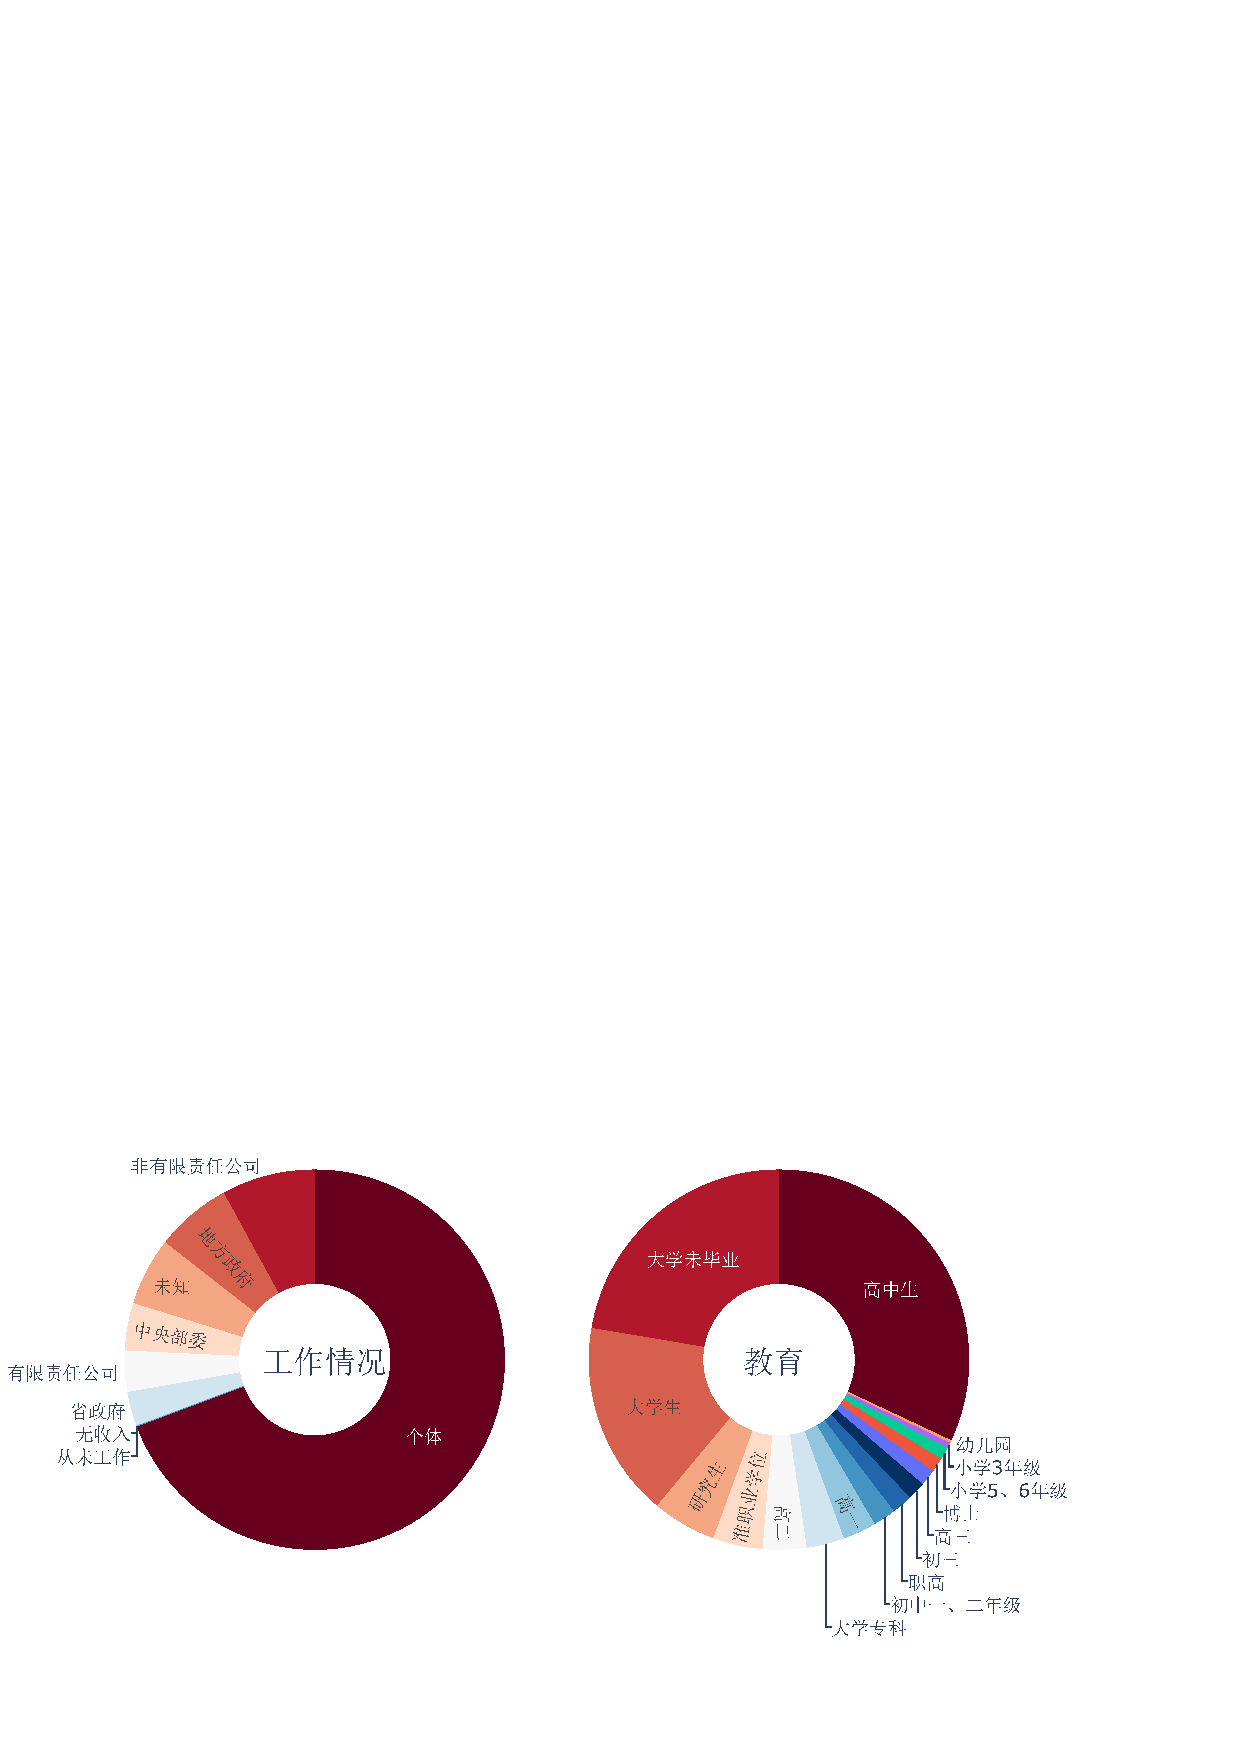
\includegraphics[width=5.0in]{images/working_education.pdf}
		\caption{Default probability against time to maturities $T$. \label{DP}}
	\end{center}
\end{figure}

\begin{figure}
	\begin{center}
		\makeatletter
		\def\@captype{figure}
		\makeatother
		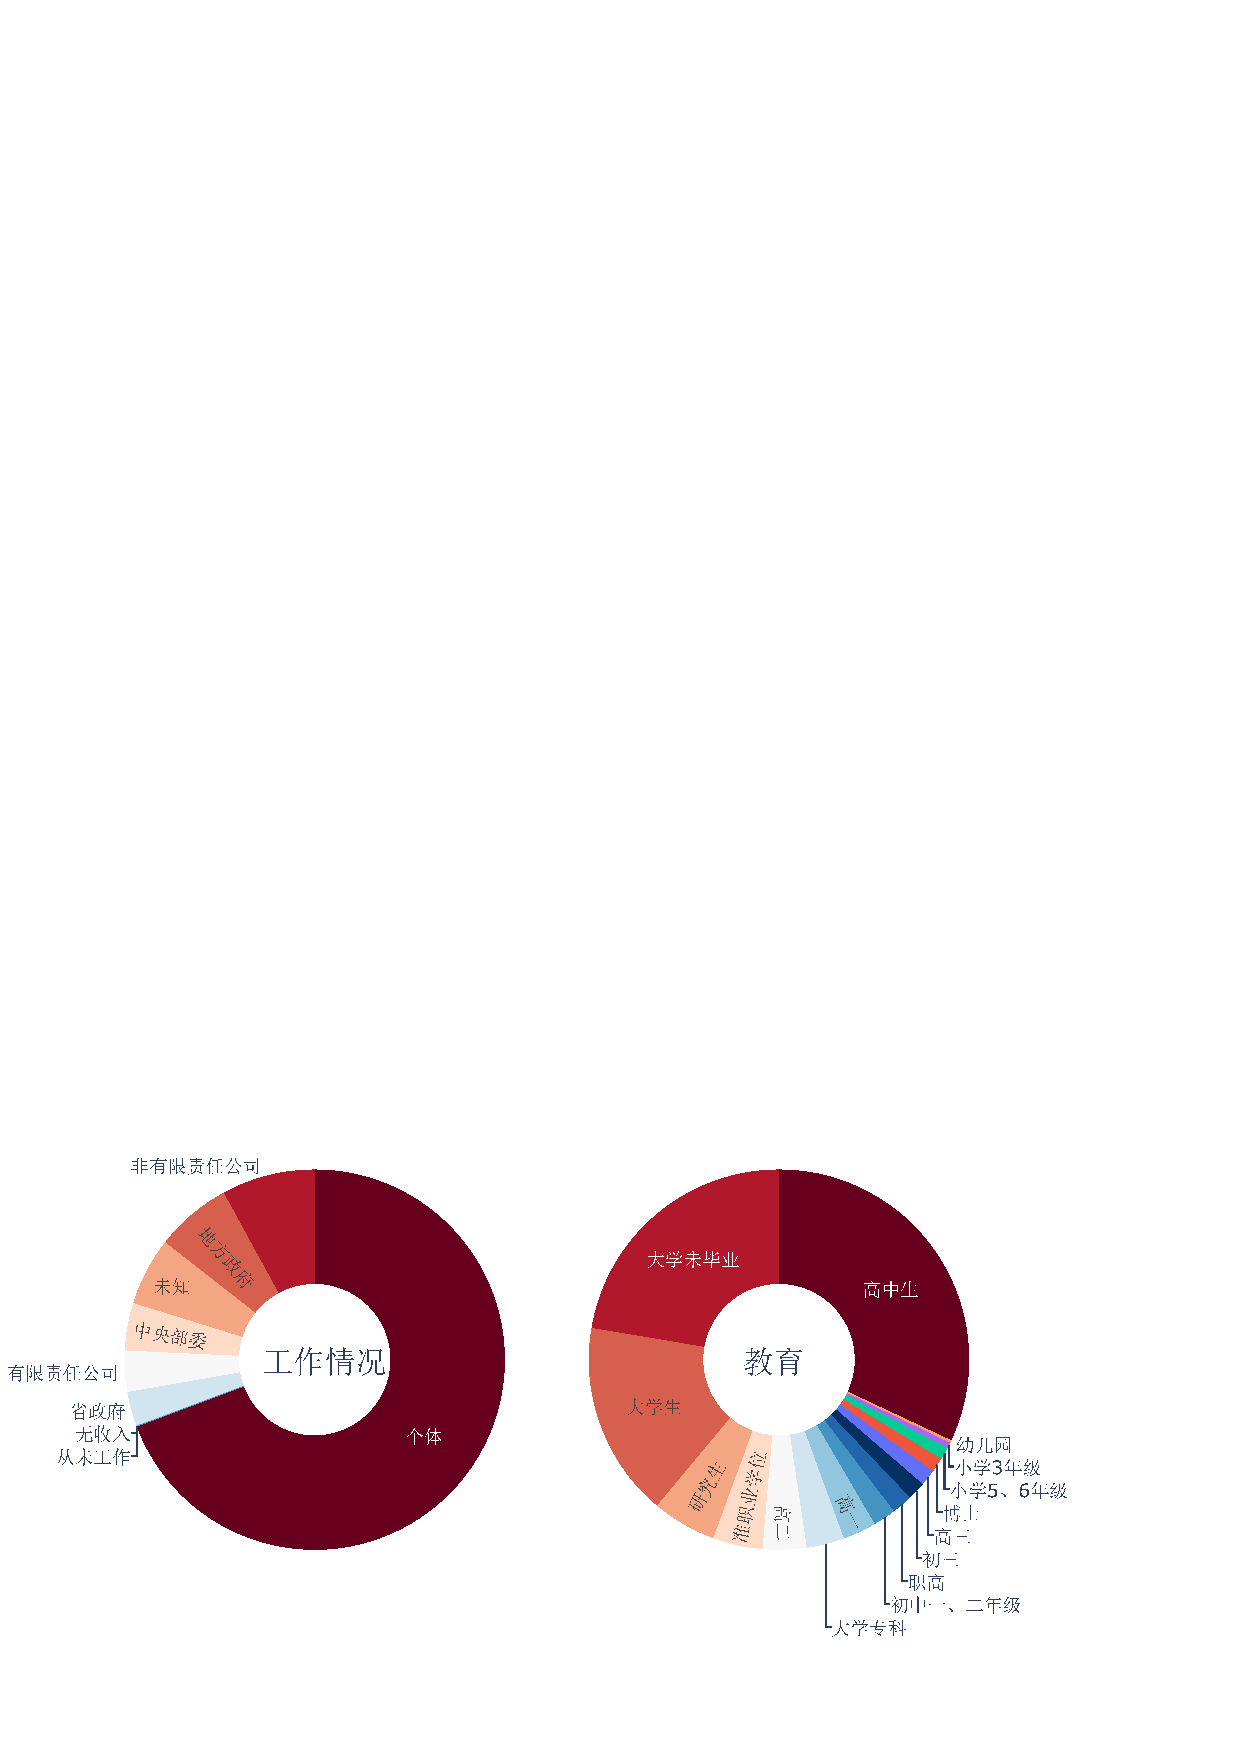
\includegraphics[width=5.0in]{images/working_education.pdf}
		\caption{Default probability against time to maturities $T$. \label{DP}}
	\end{center}
\end{figure}






















\end{document}



